\section{Case Study I: SIR}
\label{sec:case_SIR}

As first use-case we discuss property-based testing for the agent-based SIR model. It is a very well studied and understood compartment model from epidemiology \cite{kermack_contribution_1927} which allows to simulate the dynamics of an infectious disease like influenza, tuberculosis, chicken pox, rubella and measles spreading through a population.

In this model, people in a population of size $N$ can be in either one of three states \textit{Susceptible}, \textit{Infected} or \textit{Recovered} at a particular time, where it is assumed that initially there is at least one infected person in the population. People interact \textit{on average} with a given rate of $\beta$ other people per time-unit and become infected with a given probability $\gamma$ when interacting with an infected person. When infected, a person recovers \textit{on average} after $\delta$ time-units and is then immune to further infections. An interaction between infected persons does not lead to re-infection, thus these interactions are ignored in this model. The models origin is in System Dynamics (SD) \cite{porter_industrial_1962} and can be formalized in SD with the following equations:

\begin{equation}
\frac{\mathrm d S}{\mathrm d t} = -infectionRate \\ 
\frac{\mathrm d I}{\mathrm d t} = infectionRate - recoveryRate \\ 
\frac{\mathrm d R}{\mathrm d t} = recoveryRate 
\end{equation}

\begin{equation}
infectionRate = \frac{I \beta S \gamma}{N} \\
recoveryRate = \frac{I}{\delta} 
\end{equation}

%Solving these equations is done by numerically integrating over time which results in the dynamics as shown in Figure \ref{fig:sir_sd_dynamics} with the given variables.
%
%\begin{figure}
%	\centering
%	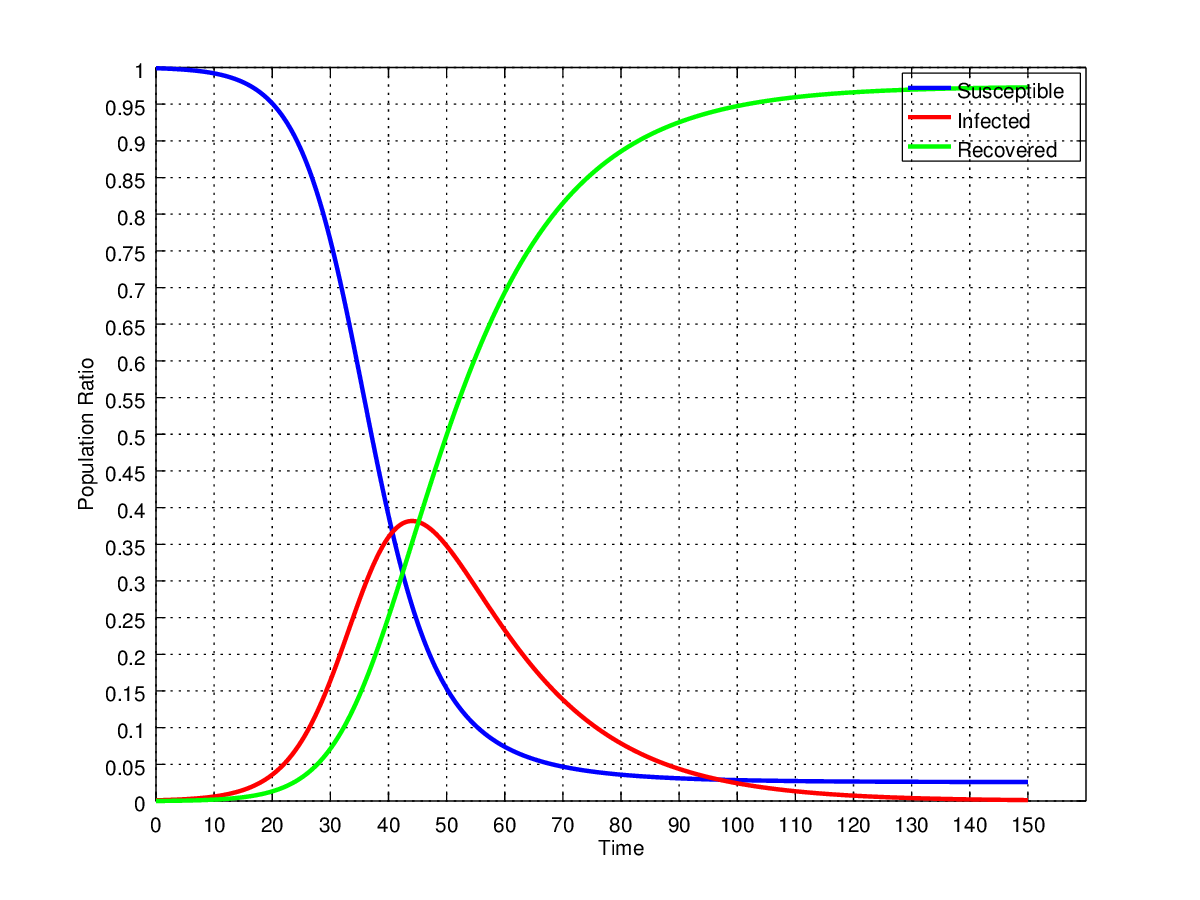
\includegraphics[width=0.3\textwidth, angle=0]{./fig/step3_dataflow/SIR_SD_1000agents_150t_001dt.png}
%	\caption{Dynamics of the SIR compartment model using the System Dynamics approach. Population Size $N$ = 1,000, contact rate $\beta =  \frac{1}{5}$, infection probability $\gamma = 0.05$, illness duration $\delta = 15$ with initially 1 infected agent. Simulation run for 150 time-steps.}
%	\label{fig:sir_sd_dynamics}
%\end{figure}

We implemented an agent-based version of this model \footnote{The code is freely accessible from \url{https://github.com/thalerjonathan/phd/tree/master/public/propabs/sir}}, which is inspired by \cite{macal_agent-based_2010}. In our property-based tests we test if the \textit{isolated} behaviour of an agent in all three states Susceptible, Infected and Recovered, corresponds to model specifications. The crucial thing though is that we are dealing with a stochastic system where the agents act \textit{on averages}, which means we need to average our tests as well 

\subsection{Susceptible Behaviour}
A susceptible agent \textit{may} become infected, depending on the number of infected agents in relation to non-infected the susceptible agent has contact to. To make this property testable we run a susceptible agent for 1.0 time-unit (note that we are sampling the system with a much smaller $\Delta t = 0.1$) and then check if it is infected - that is it returns infected as its current state. 

Obviously we need to pay attention to the fact that we are dealing with a stochastic system thus we can only talk about averages and thus it does not suffice to only run a single agent but we are repeating this for e.g. $N = 10.000$ agents (all with different random-number seeds). We then need a formula for the required fraction of the N agents which should have become infected on average. Per 1.0 time-unit, a susceptible agent makes \textit{on average} contact with $\beta$ other agents where in the case of a contact with an infected agent the susceptible agent becomes infected with a given probability $\gamma$. In this description there is another probability hidden, which is the probability of making contact with an infected agent which is simply the ratio of number of infected agents to number not infected agents. The formula for the target fraction of agents which become infected is then: $\beta * \gamma * \frac{number of infected}{number of non-infected}$. To check whether this test has passed we compare the required amount of agents which on average should become infected to the one from our tests (simply count the agents which got infected and divide by N) and if the value lies within some small $\epsilon$ then we accept the test as passed - alternatively we can implement a t-test to check this property in a more statistically robust way but this is not the point.
The input to the susceptible agents which we can vary is the set of agents with which the susceptible agents make contact with. We use property-testing with QuickCheck which creates them randomly for us and reduces them also to all relevant edge-cases.

TODO: clearly state the property we test

When we look at the formula we can see that it is a slightly different representation of the \textit{infection rate} of the SD specification as shown above. This is the very power which property-based testing offers us: we directly express the specification of the original SD model in the tests of our agent-based implementation and let QuickCheck generate random test cases for us. This closely ties our implementation to the original specification and "proves" that it is actually a valid implementation of it.

\subsection{Infected Behaviour}
An infected agent will \textit{always} recover after some finite time, which is \textit{on average} after $\delta$ time-units. Note that this property involves stochastics too, so to test this property we run a large number of infected agents e.g. $N = 10.000$ (all with different random-number seeds) until they recover, record the time of each agents recovery and then average over all recovery times. To check whether this test has passed we compare the average recovery times to $\delta$ and if they lie within some small $\epsilon$ then we accept the test as passed (note again that we could use a t-test for better stochastic robustness but this is not the point of this paper).

TODO: clearly state the property we test

in the infected agent test we check if the average duration is as specified. does this resemble the recovery rate? or in other words: can we somehow test the recovery rate?
durationsAvg = sum durations / fromIntegral (length durations)

We use property-testing with QuickCheck in this case as well to generate the set of other agents as input for the infected agents. Strictly speaking this would not be necessary as an infected agent never makes contact with other agents and simply ignores them - we could as well just feed in an empty list. We opted for using QuickCheck for the following reasons:

\begin{itemize}
	\item We wanted to stick to the interface specification of the agent-implementation as close as possible which asks to pass the states of all agents as input.
	\item We shouldn't make any assumptions about the actual implementation and if it REALLY ignores the other agents, so we strictly stick to the interface which requires us to input the states of all the other agents.
	\item The set of other agents is ignored when determining whether the test has failed or not which indicates by construction that the behaviour of an infected agent does not depend on other agents.
	\item We are not just running a single replication over 10.000 agents but 100 of them which should give black-box verification more strength.
\end{itemize}

\subsection{Recovered Behaviour}
A recovered agent will stay recovered \textit{forever}. Obviously we cannot write a property-based test that truly verifies that because it had to run in fact \textit{forever}. In this case we need to resort to white-box verification and look directly at the code and reason whether this property holds true.